\section*{Problem 3 LTI}
\subsection*{Frequency response}
Let $\dot{y}(t) + 3y(t) = x(t)$ be some LTI system.

We can solve the difference equation by using the Fourier transform.
\begin{align}
    \dot{y}(t) + 3y(t) &= x(t)\\
\Rightarrow j\omega Y(j\omega) + 3Y(j\omega) &= X(j\omega).
\end{align}

We now have eliminated the differential and can simply rearange as such
\begin{align}
   Y(j\omega)(j\omega  + 3) &= X(j\omega)\\ 
\Rightarrow \frac{Y(j\omega)}{X(j\omega)} &\equiv H(j\omega) = \frac{1}{j\omega + 3}
\end{align}

\subsection*{Bode plot}
You could just compute a few values and then sketch it by hand. Otherwise, here
is some code that does it.

\begin{lstlisting}[language=python]
# imports
import numpy as np
import matplotlib.pyplot as plt


# frequencies
ws = np.linspace(0, np.pi, 100)

# analytical frequency response
def f_rsp(w):
    return 1 / (1j * w + 3)
    
# convert to dB
def dB(s):
    return 20*np.log10(s)

# plot
fig, ax = plt.subplots()
ax.plot(ws, np.abs(f_rsp(ws)))
ax.set_title("Bode plot")
ax.set_xlabel(r"$\omega$")

plt.savefig("figures/p3_bode.png")
plt.show()
\end{lstlisting}

\begin{figure}[h!]
    \begin{center}
        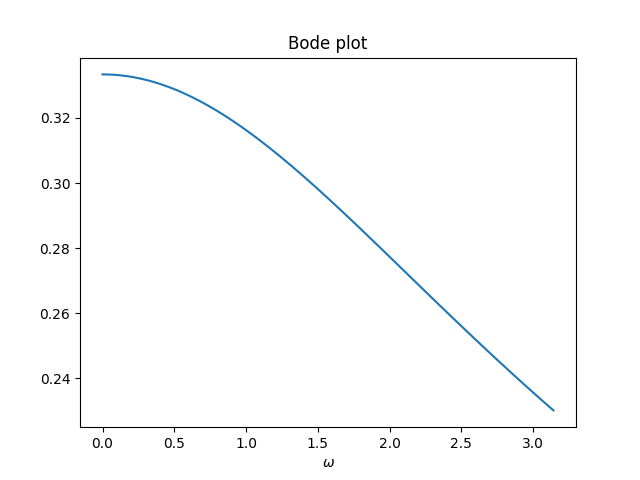
\includegraphics[width=0.75\textwidth]{figures/p3_bode.png}
    \end{center}
    \caption{Bode plot of system.}
\end{figure}

